\documentclass[ignorenonframetext,]{beamer}
\usepackage{amssymb,amsmath}
\usepackage{ifxetex,ifluatex}
\usepackage{fixltx2e} % provides \textsubscript
\usepackage{lmodern}
\ifxetex
  \usepackage{fontspec,xltxtra,xunicode}
  \defaultfontfeatures{Mapping=tex-text,Scale=MatchLowercase}
  \newcommand{\euro}{€}
\else
  \ifluatex
    \usepackage{fontspec}
    \defaultfontfeatures{Mapping=tex-text,Scale=MatchLowercase}
    \newcommand{\euro}{€}
  \else
    \usepackage[T1]{fontenc}
    \usepackage[utf8]{inputenc}
      \fi
\fi
\IfFileExists{upquote.sty}{\usepackage{upquote}}{}
% use microtype if available
\IfFileExists{microtype.sty}{\usepackage{microtype}}{}
\usepackage{letltxmacro}
\makeatletter
\def\maxwidth{\ifdim\Gin@nat@width>\linewidth\linewidth\else\Gin@nat@width\fi}
\def\maxheight{\ifdim\Gin@nat@height>\textheight0.8\textheight\else\Gin@nat@height\fi}
\makeatother
\AtBeginDocument{
  \LetLtxMacro\Oldincludegraphics\includegraphics
  \renewcommand{\includegraphics}[2][]{%
    \Oldincludegraphics[#1,width=\maxwidth,height=\maxheight,keepaspectratio]{#2}}
}

% Comment these out if you don't want a slide with just the
% part/section/subsection/subsubsection title:
\AtBeginPart{
  \let\insertpartnumber\relax
  \let\partname\relax
  \frame{\partpage}
}
\AtBeginSection{
  \let\insertsectionnumber\relax
  \let\sectionname\relax
  \frame{\sectionpage}
}
\AtBeginSubsection{
  \let\insertsubsectionnumber\relax
  \let\subsectionname\relax
  \frame{\subsectionpage}
}

\setlength{\parindent}{0pt}
\setlength{\parskip}{6pt plus 2pt minus 1pt}
\setlength{\emergencystretch}{3em}  % prevent overfull lines
\setcounter{secnumdepth}{0}

\title{Missing Sticks: Property Institutions and Income Dissipation in Indian
Country}
\author{Jacob W. Russ (with Thomas Stratmann)}
\date{February 6th, 2014}

\begin{document}
\frame{\titlepage}

\begin{frame}{Introduction}

\begin{itemize}
\item
  We study the effect of property rights and institutions for economic
  growth and development.
\item
  Application: Estimate the effect of missing property rights on Indian
  reservations on Indian income.
\end{itemize}

\end{frame}

\begin{frame}{Institutions: Land Ownership Rights}

\begin{itemize}
\itemsep1pt\parskip0pt\parsep0pt
\item
  Indians do not control the legal titles to their land parcels

  \begin{itemize}
  \item
    Titles to land parcels are held in federal trust with Indians as
    beneficiaries
  \item
    Indian owners cannot unilaterally perform ordinary real estate
    transactions (sell, mortgage, lease, etc.)
  \item
    It is the Bureau of Indian Affairs (BIA) policy not to approve any
    Indian land sales, thus no alienation of ownership claims is
    possible
  \end{itemize}
\end{itemize}

\end{frame}

\begin{frame}{Institutions cont.}

\begin{itemize}
\itemsep1pt\parskip0pt\parsep0pt
\item
  BIA probates the estates of deceased Indians

  \begin{itemize}
  \itemsep1pt\parskip0pt\parsep0pt
  \item
    Originally Indian wills were not recognized and wills remain outside
    the cultural norms of Indians
  \end{itemize}
\item
  In the absence of a will, heirs typically obtain an equal fraction of
  the deceased's land interests.

  \begin{itemize}
  \itemsep1pt\parskip0pt\parsep0pt
  \item
    Leads to Indian land fractionation
  \end{itemize}
\item
  Land ownership is shared as ``tenants in common''

  \begin{itemize}
  \itemsep1pt\parskip0pt\parsep0pt
  \item
    Indian co-owners share percentages of the whole parcel, not
    identifiable (physical) sections of land
  \end{itemize}
\end{itemize}

\end{frame}

\begin{frame}{Fractionation Illustrated}

\centering
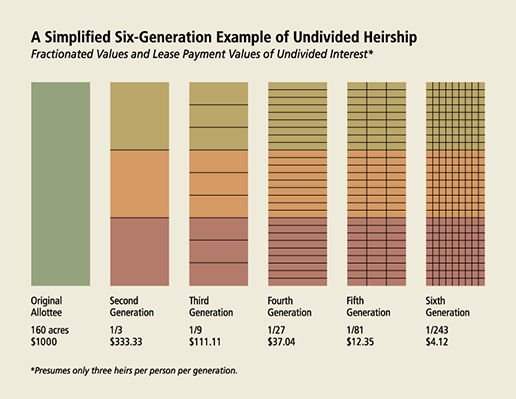
\includegraphics{heirship-new-opt.png}

\end{frame}

\begin{frame}{Data}

\begin{itemize}
\itemsep1pt\parskip0pt\parsep0pt
\item
  Trust Asset and Accounting Management System (TAAMS)

  \begin{itemize}
  \itemsep1pt\parskip0pt\parsep0pt
  \item
    Cross-section of all trust land areas (reservations) in April 2010
  \item
    Anonymized system reference number for ownership id
  \item
    Agricultural lease income
  \end{itemize}
\item
  ``Current'' state of the Federal Indian Trust

  \begin{itemize}
  \itemsep1pt\parskip0pt\parsep0pt
  \item
    270,000 Indian owners with 4.6 million Indian ownership records\\
  \item
    An average of \textasciitilde{} 17 ownership records per Indian
    owner
  \end{itemize}
\end{itemize}

\end{frame}

\begin{frame}{Hypotheses}

\begin{itemize}
\item
  Fractionation increases transaction costs/bargaining costs as to how
  to use the land
\item
  Implication: Reservations that contain land with higher levels of
  fractionation will have lower levels of income because of the costs
  and difficulties of coming to an agreement for how to use the land
\end{itemize}

\end{frame}

\begin{frame}{Reservation Level Empirical Model}

\[ IndianIncome_{i} = \alpha Fractionation_{i} + \delta X_{i} + \varepsilon _{i}\]

\begin{itemize}
\itemsep1pt\parskip0pt\parsep0pt
\item
  Fractionation is measured as the number of (consolidated) ownership
  interests on a reservation
\item
  Controls: surface acres, percent fee, percent Indian, percent
  completed high school
\end{itemize}

\end{frame}

\begin{frame}{Reservation: Median Household Income}

\centering
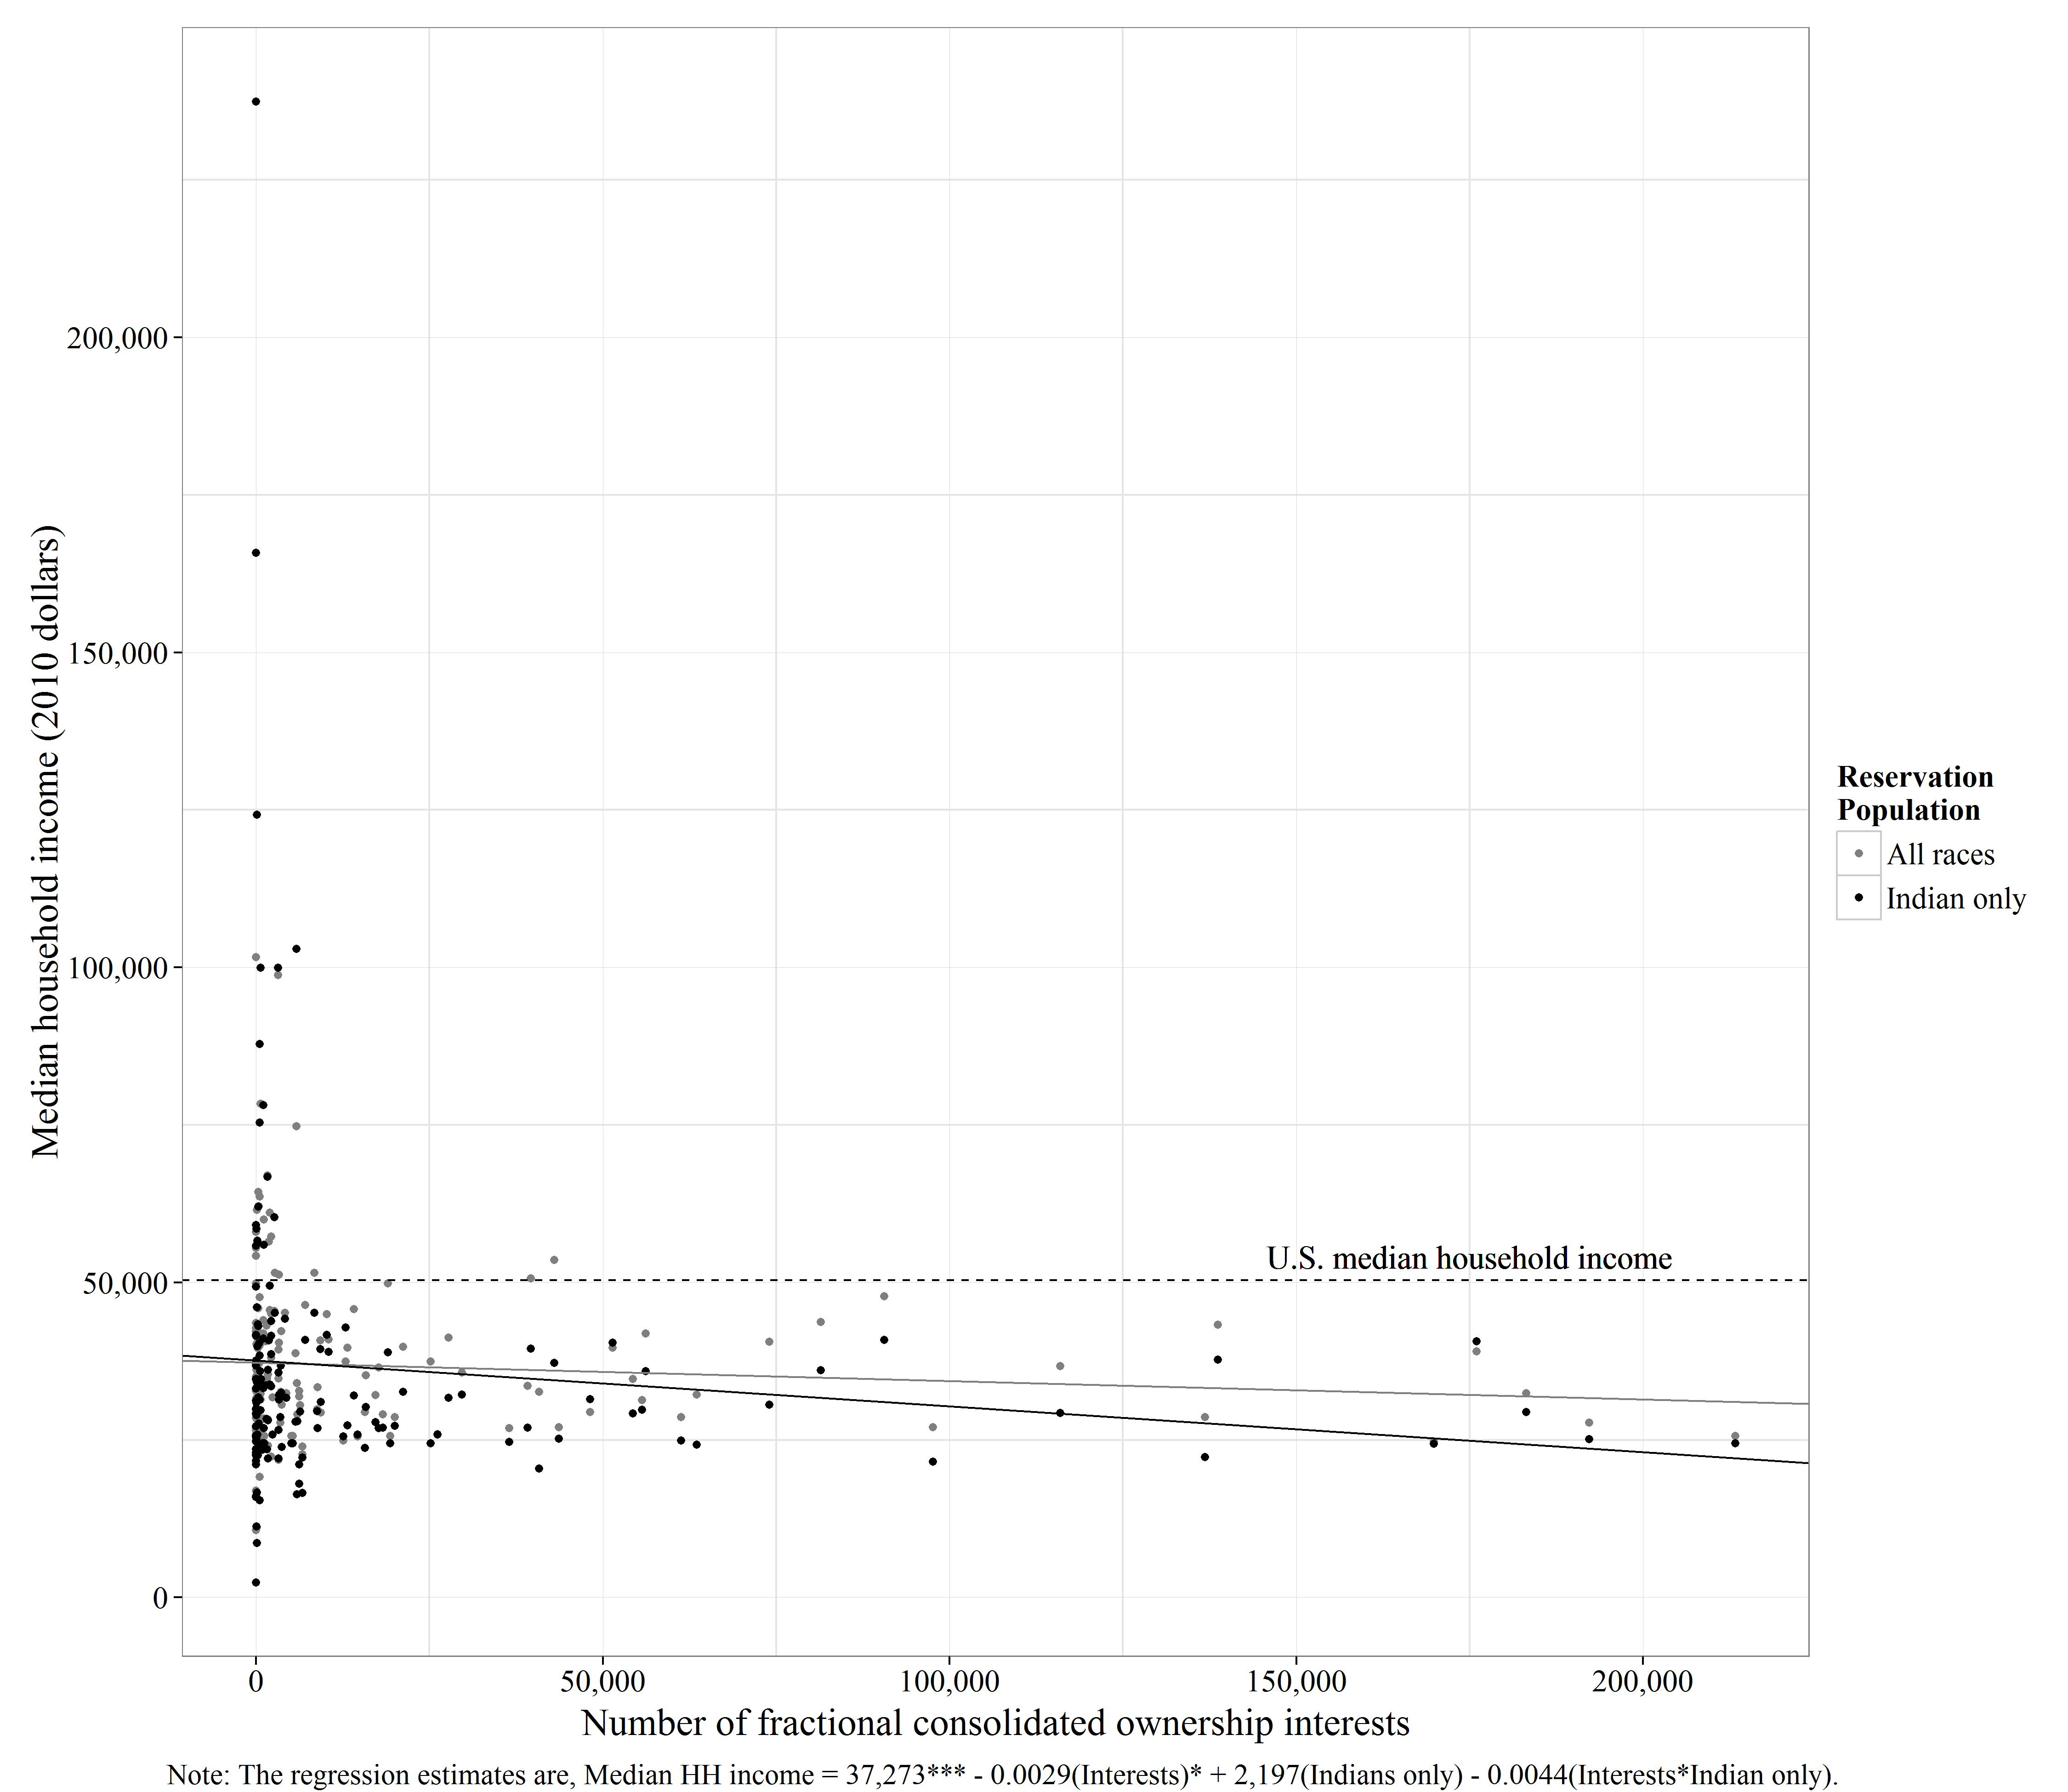
\includegraphics{frac_med_hh_inc.jpeg}

\end{frame}

\begin{frame}{Reservation: Per Capita Income}

\centering
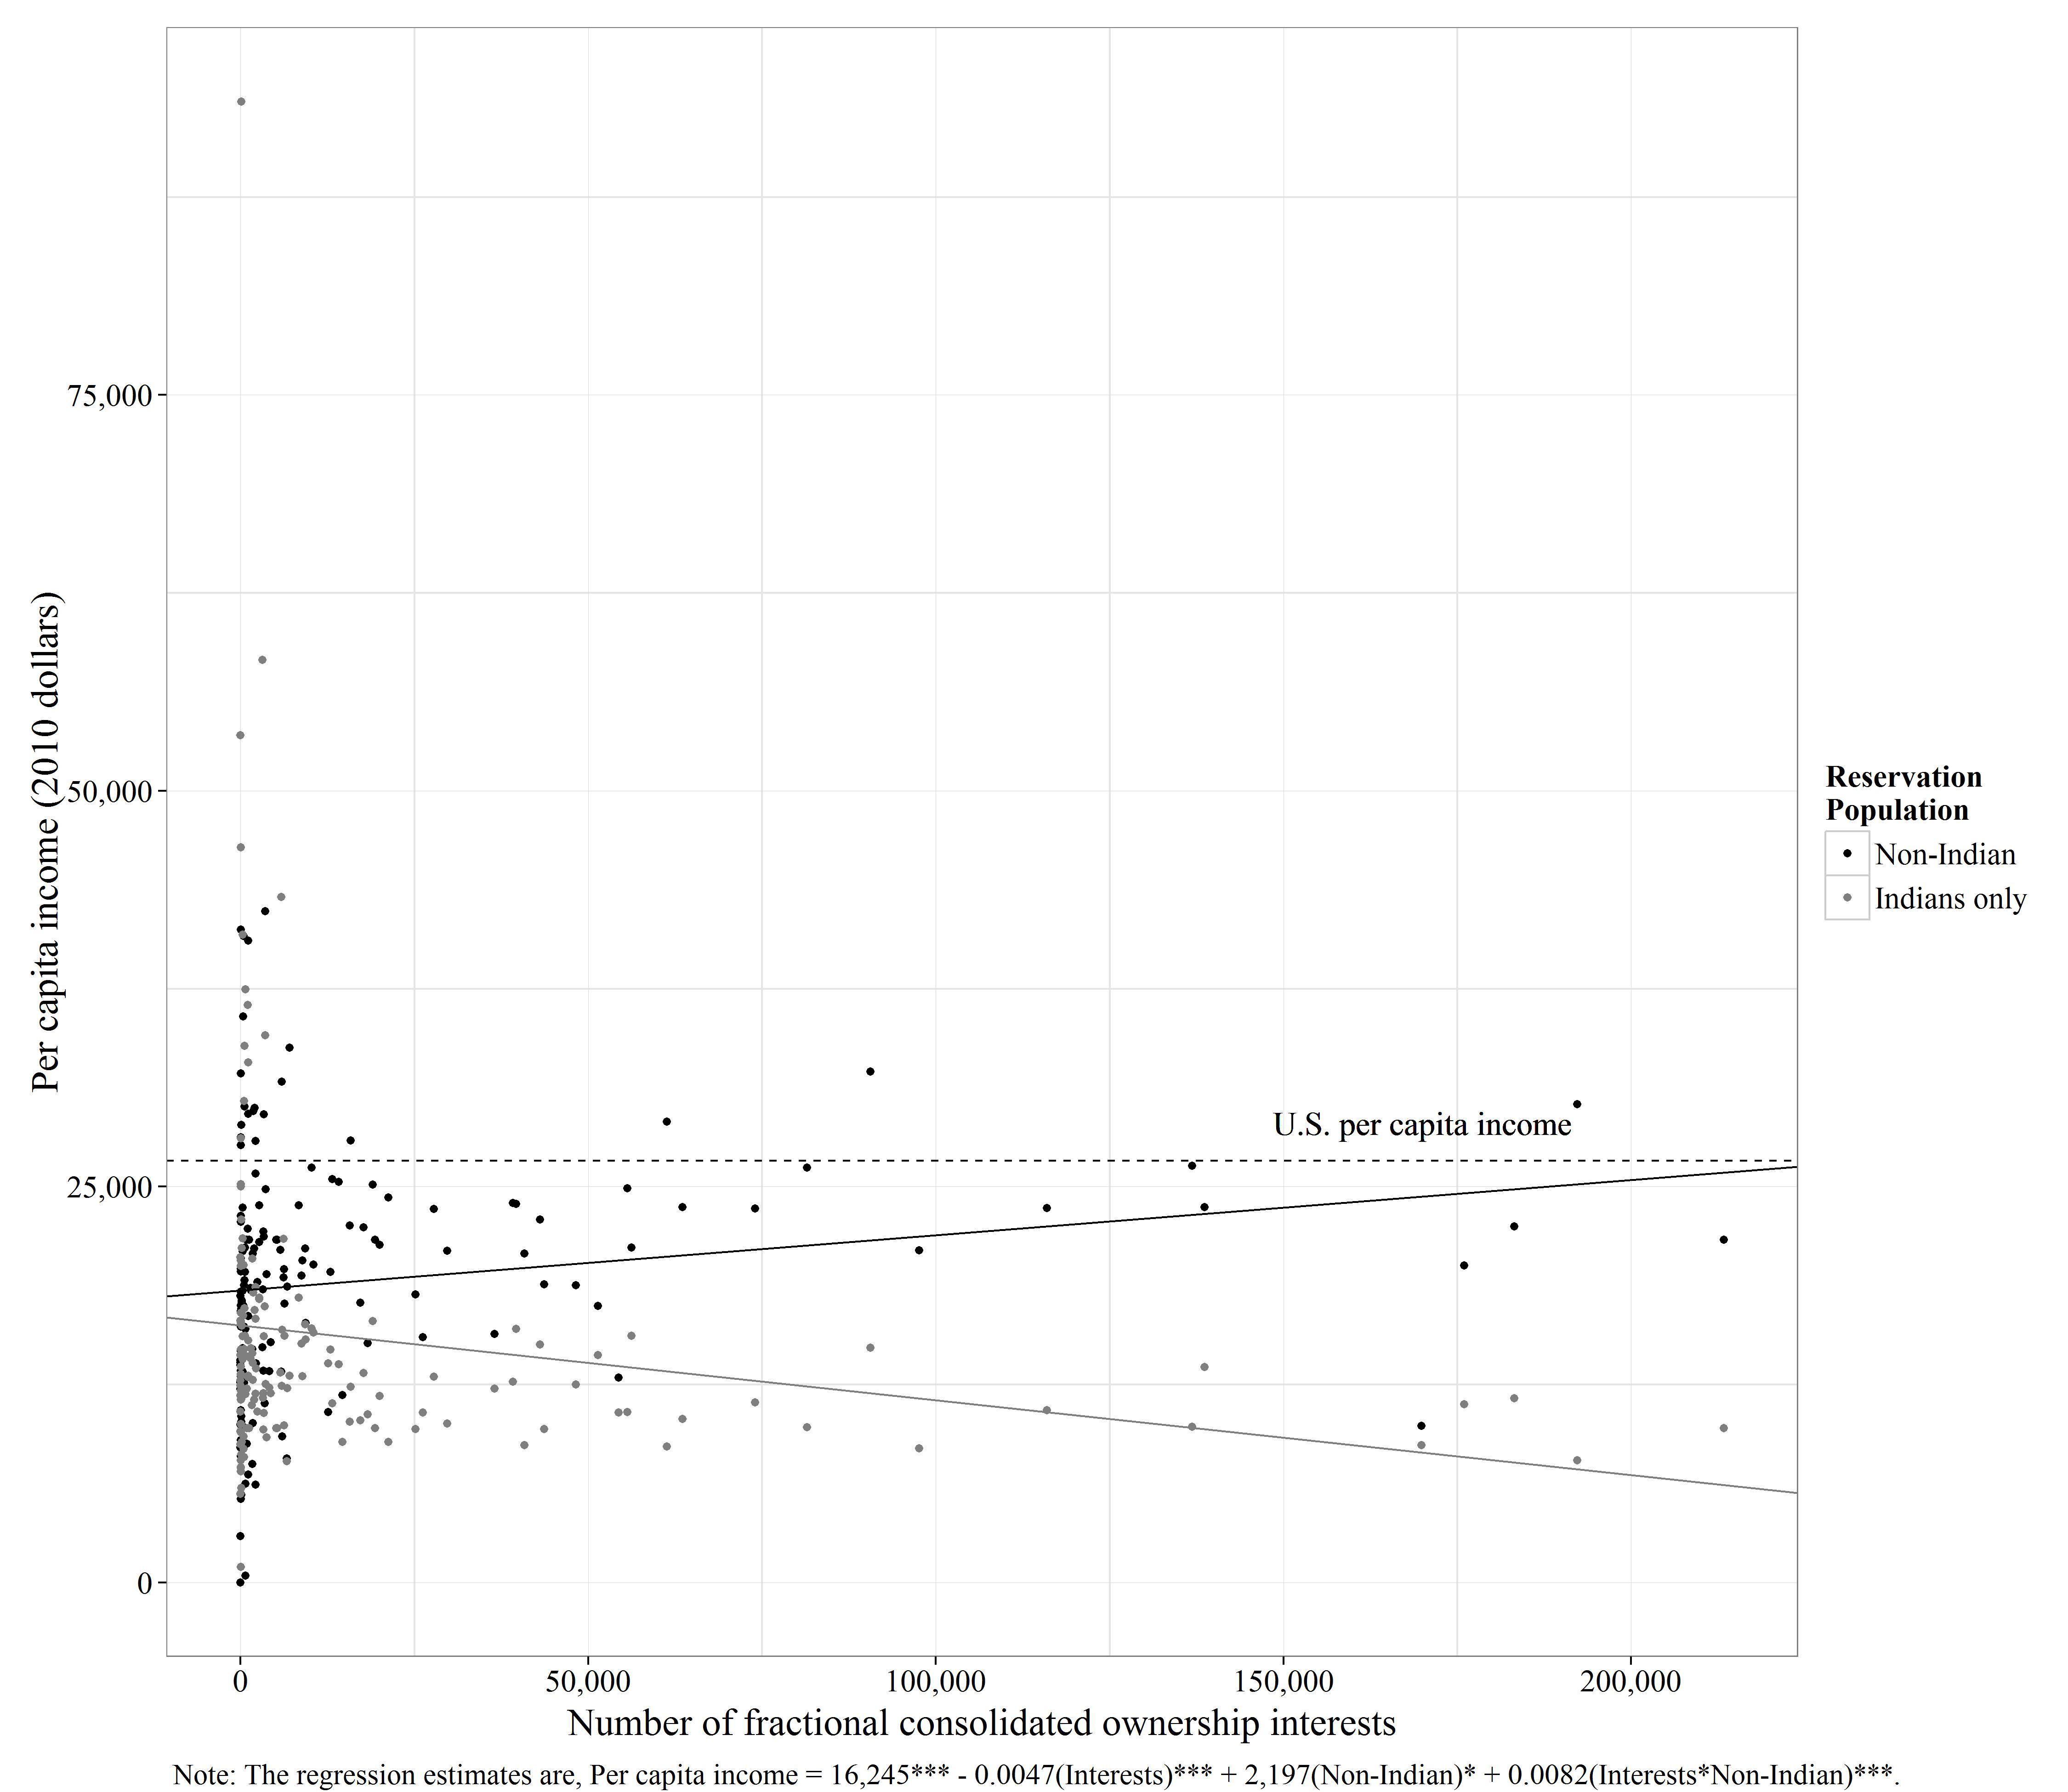
\includegraphics{frac_pcinc.jpeg}

\end{frame}

\begin{frame}{Causal Effect?}

\begin{itemize}
\itemsep1pt\parskip0pt\parsep0pt
\item
  Instrument: Number of allotments approved by BIA (Dept. of Indian
  Affairs) between 1860 and 1934.

  \begin{itemize}
  \itemsep1pt\parskip0pt\parsep0pt
  \item
    More allotments on a reservation means a larger population, thus
    fractionation is likely to progress faster.
  \end{itemize}
\item
  IV findings: Same sign and statistical significance as when estimating
  with OLS
\end{itemize}

\end{frame}

\begin{frame}{Reservation IV Models}

\centering
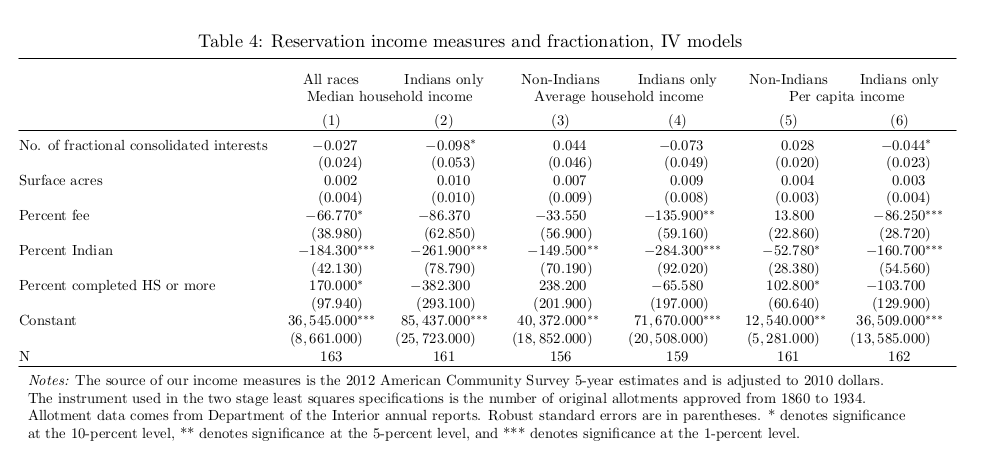
\includegraphics{Table4.png}

\end{frame}

\begin{frame}{Institutions: Leasing Trust Land}

\begin{itemize}
\item
  For trust property to be ``employed'', BIA requires a lease or
  permission from co-owners
\item
  Leasing is conditional on BIA approval

  \begin{itemize}
  \itemsep1pt\parskip0pt\parsep0pt
  \item
    Majority ownership required to initiate a privately directed lease,
    a costly activity and BIA approval process is slow
  \end{itemize}
\item
  BIA has responsibility to attempt to lease land which would ``lie
  fallow'' (when there is no Indian directed lease)
\end{itemize}

\end{frame}

\begin{frame}{Principal Agent Issues}

\begin{itemize}
\item
  \textbf{Principal:} Indians\\
\item
  \textbf{Agent:} BIA
\item
  BIA leases tracts and there is anecdotal evidence that BIA does not
  get maximal possible lease rates

  \begin{itemize}
  \itemsep1pt\parskip0pt\parsep0pt
  \item
    Each owner has less of an incentive to monitor that the BIA obtains
    market rate for leasing, when there are more owners per acre of a
    given tract.
  \end{itemize}
\end{itemize}

\end{frame}

\begin{frame}{Model of ag land leasing}

\centering
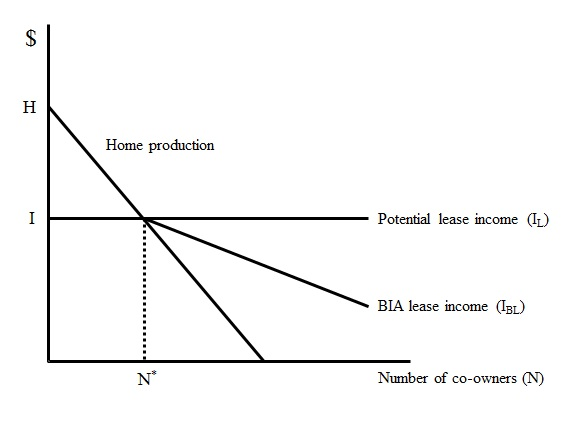
\includegraphics{model.jpeg}

\end{frame}

\begin{frame}{Hypotheses}

\begin{itemize}
\item
  Less fractionated land is less likely to be leased through BIA
\item
  When tracts are leased though the BIA, tracts that are more
  fractionated will generate less lease income
\end{itemize}

\end{frame}

\begin{frame}{Estimation Strategy}

\begin{itemize}
\itemsep1pt\parskip0pt\parsep0pt
\item
  Linear probability model
\end{itemize}

\[ Pr(Lease = 1)_{ij} = \beta_{0} + \beta_{1}Fractionation_{ij} + \delta X_{ij} 
+ \varepsilon _{st} \]

\begin{itemize}
\item
  Fractionation is measured as the number of owners of a given parcel\\
\item
  Controls: parcel size and resource type (surface or both surface and
  subsurface)
\item
  Agricultural lease income model
\end{itemize}

\[ LeaseIncomePerAcre_{ij} = \beta_{0} + \beta_{1}Fractionation_{ij} + \delta X_{ij} 
+ \varepsilon _{st} \]

\end{frame}

\begin{frame}{Results Linear Probability Models}

\centering
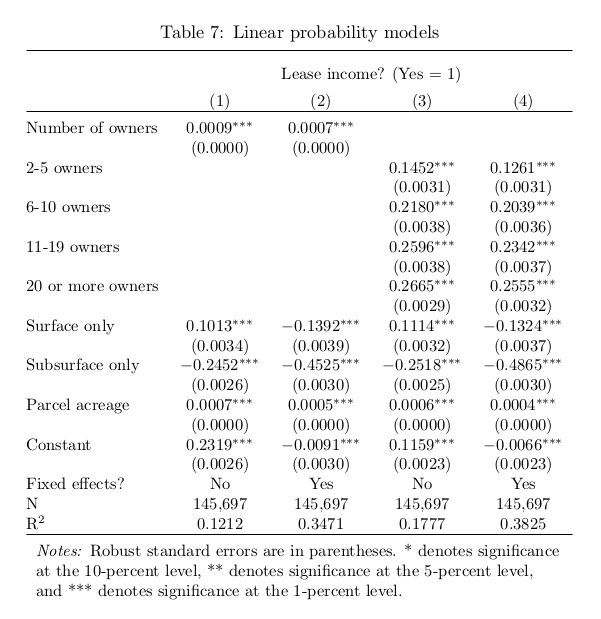
\includegraphics{Table7.png}

\end{frame}

\begin{frame}{Results Agricultural Income Models}

\centering
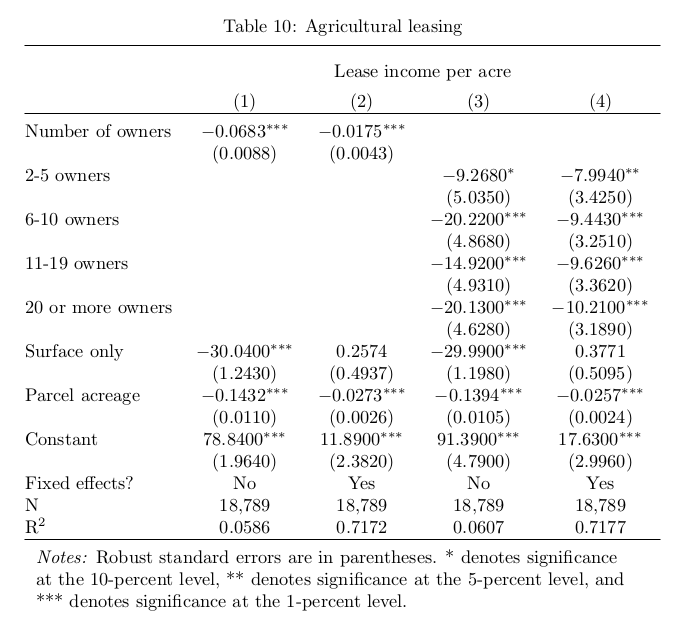
\includegraphics{Table10.png}

\end{frame}

\begin{frame}{Findings}

\begin{itemize}
\item
  Fractionation leads to lower Indian incomes on reservations.

  \begin{itemize}
  \itemsep1pt\parskip0pt\parsep0pt
  \item
    We suggest that the underlying mechanism is that incomplete property
    rights increase the transaction costs for Indian landowners.
  \end{itemize}
\item
  BIA leasing of land is subject to principal agent issues
\item
  We estimate that fractionation reduces the annual agricultural lease
  income by between \$3,962 and \$5,062 per parcel per year.
\item
  Parcels with 20+ owners lease are twice as likely to be leased as
  those with 2-5 owners.
\end{itemize}

\end{frame}

\begin{frame}

\begin{center}

\huge{Thank you!}

\end{center}

\end{frame}

\end{document}
